\documentclass[11pt,a4paper]{article}

\usepackage[margin=1in]{geometry}
\usepackage[T1]{fontenc}
\usepackage{lmodern}
\usepackage{microtype}
\usepackage{amsmath,amssymb}
\usepackage{booktabs}
\usepackage{longtable}
\usepackage{array}
\usepackage{enumitem}
\usepackage{hyperref}
\usepackage{xcolor}
\usepackage{tikz}
\usetikzlibrary{arrows.meta,positioning,fit,calc,shapes.multipart}

\hypersetup{colorlinks=true,linkcolor=blue,urlcolor=blue,citecolor=blue}
\setlist[itemize]{leftmargin=*,noitemsep,topsep=3pt}
\setlist[enumerate]{leftmargin=*,itemsep=3pt,topsep=3pt}

\title{UMLCAD V5\\Software Architecture}
\author{UMLCAD Project}
\date{September 2026}

\newcommand{\UMLCAD}{UMLCAD}
\newcommand{\Kernel}{CAD Kernel}
\newcommand{\Router}{Routing Server}
\newcommand{\GitServer}{Git Server}
\newcommand{\CADAPI}{CAD API}

\begin{document}
\maketitle
\tableofcontents
\newpage

\section{Purpose and Architectural Intent}

UMLCAD V5 is a code-driven CAD system in which engineering design is authored as source code. The source program is evaluated by a CAD framework and kernel, producing validated engineering results and standard downstream artifacts. A browser application provides visualization and interaction; it does not become the engineering authority.

The architecture deliberately separates four concerns:
\begin{enumerate}
    \item \textbf{source and version control}: Git repositories and designer workspaces;
    \item \textbf{CAD computation}: a stable, transport-independent CAD API implemented by the UMLCAD framework and kernel;
    \item \textbf{application orchestration}: routing, process management, source editing, LLM integration, and browser communication;
    \item \textbf{presentation}: browser rendering, selection, property inspection, and user interaction.
\end{enumerate}

A primary architectural rule is:

\begin{quote}
The CAD kernel has a stable API, but it does not depend on Git, WebSocket, HTTP, browser code, authentication, an LLM, or a particular deployment topology.
\end{quote}

The CAD API is designed as a RESTful, stateless contract. Statelessness describes the external contract; the implementation may use deterministic caches and incremental evaluation internally.

\section{System Model}

The default deployment is a server containing the routing layer, a general Git service, source-editor/LLM facilities, and the CAD API infrastructure. A designer interacts only with the browser-facing application boundary.

\begin{center}
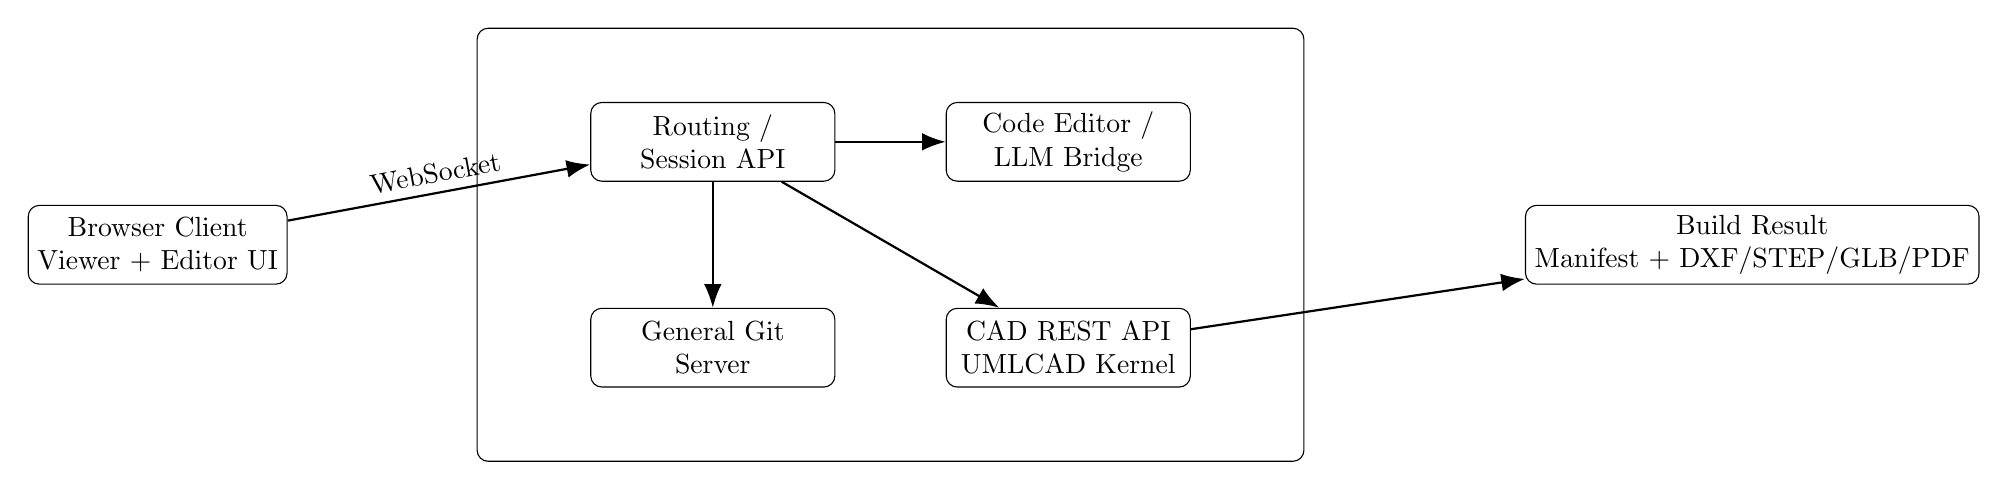
\begin{tikzpicture}[
  node distance=10mm and 14mm,
  box/.style={draw,rounded corners,align=center,minimum width=31mm,minimum height=10mm},
  big/.style={draw,rounded corners,inner sep=7mm},
  arr/.style={-{Latex[length=3mm]},thick}
]
  \node[box] (browser) {Browser Client\\Viewer + Editor UI};
  \node[big, right=24mm of browser, minimum width=105mm, minimum height=55mm] (server) {};
  \node[box, above left=8mm and 7mm of server.center] (router) {Routing /\\Session API};
  \node[box, below left=8mm and 7mm of server.center] (git) {General Git\\Server};
  \node[box, above right=8mm and 7mm of server.center] (editor) {Code Editor /\\LLM Bridge};
  \node[box, below right=8mm and 7mm of server.center] (cad) {CAD REST API\\UMLCAD Kernel};
  \node[box, right=28mm of server] (art) {Build Result\\Manifest + DXF/STEP/GLB/PDF};
  \draw[arr] (browser) -- node[above,sloped]{WebSocket} (router);
  \draw[arr] (router) -- (git);
  \draw[arr] (router) -- (editor);
  \draw[arr] (router) -- (cad);
  \draw[arr] (cad) -- (art);
\end{tikzpicture}
\end{center}

The physical components may be colocated in one server for low-latency internal communication. They remain logically separated by explicit interfaces so that later scaling or process isolation does not require redesign of the browser protocol.

\section{Architectural Boundaries}

\subsection{Browser}

The browser is the only required client application. It is responsible for:
\begin{itemize}
    \item visualization and camera operations;
    \item semantic hit testing and selection;
    \item displaying object properties and diagnostics;
    \item requesting property changes and other semantic operations;
    \item displaying process history and requesting undo/redo;
    \item interacting with the code editor UI when exposed;
    \item receiving live results and build notifications over WebSocket.
\end{itemize}

The browser does not decide engineering validity, solve constraints, own Git history, or mutate generated CAD artifacts as a substitute for source editing.

\subsection{Routing / Session API}

The routing layer is the application orchestrator. It owns the browser-facing WebSocket/session protocol and routes operations to the appropriate internal services. It may coordinate authentication context, project selection, process execution, source editing, CAD requests, and Git operations.

The routing layer must not become a second CAD engine. It does not own geometric semantics, constraint mathematics, topology, or kernel validity rules.

\subsection{General Git Server}

Git is the durable source-collaboration mechanism. Every UMLCAD project is a Git repository. Each designer has an independent clone or working copy and may experiment privately.

A designer's uncommitted source changes are private to that workspace. Colleagues do not see trial-and-error changes merely because they are connected to the same project. Committed changes become available through ordinary Git collaboration, for example through the project's update/fetch/merge workflow.

Git is not the CAD interaction API and is not required for each kernel request.

\subsection{Code Editor and LLM}

The editor/LLM subsystem modifies source code. Human editing and LLM editing are represented internally as source-edit operations.

The editor or LLM is never the engineering authority. Its output is proposed source code that must pass compilation/evaluation and kernel validation before the resulting CAD revision is accepted.

\subsection{CAD REST API}

The CAD API is the stable programmatic interface to the UMLCAD framework and kernel. The initial public contract is RESTful and stateless.

Example classes of endpoint include:
\begin{itemize}
    \item build or evaluate source;
    \item query semantic objects and properties;
    \item validate a candidate semantic operation;
    \item apply a requested operation to a supplied base revision;
    \item solve and validate a candidate model;
    \item generate semantic manifests and standard artifacts;
    \item retrieve diagnostics and build metadata.
\end{itemize}

The API is stateless in the sense that every request supplies the information necessary to reproduce the requested computation. The implementation may retain caches, compiled modules, evaluated dependency nodes, and generated artifacts. A cache miss must reduce performance, not change semantics.

\section{State Ownership}

A critical distinction is made between source history, private workspace state, and evaluated CAD state.

\begin{center}
\begin{tabular}{>{\bfseries}p{0.28\linewidth}p{0.62\linewidth}}
\toprule
Authority & Responsibility \\
\midrule
Git repository & Durable source history, commits, branches, collaboration boundary. \\
Designer workspace & Current private working tree, including uncommitted experiments. \\
CAD API / kernel & Geometric, topological, constraint, validation, and engineering truth for a supplied revision/candidate. \\
Routing layer & Session and process orchestration; not engineering truth. \\
Editor / LLM & Source modification mechanism; not engineering truth. \\
Browser & Presentation and interaction; not engineering truth. \\
\bottomrule
\end{tabular}
\end{center}

A browser may display an evaluated revision that has not yet been committed to Git. This is a private runtime state for that designer. A Git commit is a durable history event, not a prerequisite for local interactive viewing.

\section{CAD API Statelessness}

\subsection{Logical Stateless Contract}

A CAD request identifies its inputs explicitly. A typical request contains a project or workspace identifier, an immutable source revision or build identity, and a semantic operation.

For example:

\begin{verbatim}
POST /cad/operation/validate
{
  "project": "car-x",
  "baseRevision": "R842",
  "operation": {
    "kind": "property.change",
    "target": "hole-17",
    "property": "diameter",
    "value": 12
  }
}
\end{verbatim}

The service does not rely on a hidden ``current model'' associated with an HTTP session. The same request against the same immutable input must produce the same semantic result within the defined numerical tolerances.

\subsection{Internal Caching}

Statelessness does not prohibit internal state. The implementation should use content-addressed or revision-addressed caches such as:
\begin{itemize}
    \item source/module compilation results;
    \item dependency graphs;
    \item evaluated CAD nodes;
    \item solver preparation data;
    \item semantic manifests;
    \item standard CAD artifacts.
\end{itemize}

The cache is an optimization and is not an authority.

\section{Incremental Compilation and Evaluation}

Interactive CAD requires small changes to be handled without recompiling and resolving an entire project whenever possible.

The system therefore separates two optimizations.

\subsection{Incremental source compilation}

A source dependency graph identifies which source modules are affected by a change. If a designer changes one source module, unchanged modules remain reusable when the language/compiler semantics permit it.

\[
\text{source patch}
\rightarrow
\text{dependency graph}
\rightarrow
\text{changed compilation units}
\rightarrow
\text{updated program}
\]

\subsection{Incremental CAD evaluation}

After compilation, the kernel evaluates only the affected semantic dependency subgraph where possible.

\begin{center}
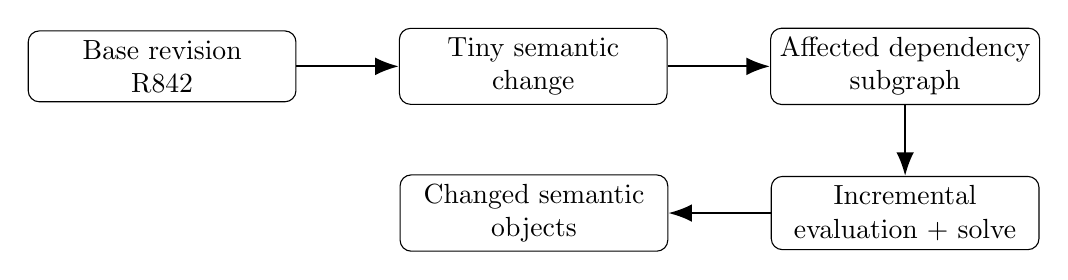
\begin{tikzpicture}[
  node distance=9mm and 13mm,
  box/.style={draw,rounded corners,align=center,minimum width=34mm,minimum height=9mm},
  arr/.style={-{Latex[length=3mm]},thick}
]
\node[box] (base) {Base revision\\R842};
\node[box,right=of base] (change) {Tiny semantic\\change};
\node[box,right=of change] (dep) {Affected dependency\\subgraph};
\node[box,below=of dep] (eval) {Incremental\\evaluation + solve};
\node[box,left=of eval] (result) {Changed semantic\\objects};
\draw[arr] (base) -- (change);
\draw[arr] (change) -- (dep);
\draw[arr] (dep) -- (eval);
\draw[arr] (eval) -- (result);
\end{tikzpicture}
\end{center}

A change may expand the affected set. Structural or global changes are allowed to fall back to a larger or full rebuild. Incrementality is therefore an optimization strategy governed by dependency analysis, not an artificial requirement that every change remain local.

\subsection{Revision-addressed incremental operation}

A request may identify a base revision and a semantic change. Internally, the kernel may reuse cached information for the base revision and derive a new revision without reconstructing unaffected work.

\[
R_{n} + \Delta \rightarrow R_{n+1}
\]

where $\Delta$ is the requested semantic operation and $R_{n+1}$ is accepted only after validation.

\section{Kernel Computational Contract}

The kernel API exposes an engineering computation model rather than a UI model. Representative operations are:
\begin{itemize}
    \item resolve or query stable semantic object identities;
    \item query properties, geometry, topology, constraints, and dependencies;
    \item evaluate candidate operations;
    \item solve constraints;
    \item regenerate affected model regions;
    \item validate geometry, topology, references, and engineering rules;
    \item produce deterministic semantic projections and artifact data.
\end{itemize}

The kernel has one engineering geometry authority. SVG, DXF, STEP, GLB, PDF, screen coordinates, and browser state are projections or consumers and must not become alternative authorities.

\section{Semantic CAD Result}

A successful build produces standard CAD artifacts together with a UMLCAD semantic manifest.

The manifest is not a second geometry database. It binds UMLCAD semantics to the authoritative kernel result. It may contain:
\begin{itemize}
    \item stable object identities;
    \item object type/kind;
    \item component definition and instance identities;
    \item source/provenance bindings;
    \item typed properties and units;
    \item editability and interaction capabilities;
    \item geometry/topology references where reliable;
    \item constraint associations;
    \item parent/child relationships;
    \item diagnostics;
    \item build and revision identity.
\end{itemize}

\subsection{Standard artifact targets}

The first target mapping is:
\begin{itemize}
    \item 2D engineering drawing: DXF;
    \item 3D mechanical CAD: STEP AP242;
    \item browser-oriented 3D visualization: GLB/glTF when appropriate;
    \item document/print output: PDF.
\end{itemize}

The artifact format must never be asked to represent engineering semantics that the kernel itself does not own.

\section{Interactive Operation and Validation}

A browser property edit follows a transactional process.

\begin{center}
\begin{tikzpicture}[
  node distance=7mm and 11mm,
  box/.style={draw,rounded corners,align=center,minimum width=35mm,minimum height=9mm},
  decision/.style={diamond,draw,aspect=2,align=center,inner sep=1pt},
  arr/.style={-{Latex[length=3mm]},thick}
]
\node[box] (intent) {Browser semantic intent};
\node[box,right=of intent] (route) {Routing layer};
\node[box,right=of route] (candidate) {Kernel candidate\\validation};
\node[decision,right=of candidate] (ok) {Accepted?};
\node[box,below=of ok] (edit) {Source edit\\(human/LLM)};
\node[box,left=of edit] (build) {Compile + incremental\\CAD evaluation};
\node[box,left=of build] (final) {Final kernel\\validation};
\node[decision,left=of final] (valid) {Valid?};
\node[box,below=of valid] (commit) {Commit process\\to live workspace state};
\node[box,right=of valid] (reject) {Reject /\\rollback};
\draw[arr] (intent) -- (route);
\draw[arr] (route) -- (candidate);
\draw[arr] (candidate) -- (ok);
\draw[arr] (ok) -- node[right]{yes} (edit);
\draw[arr] (edit) -- (build);
\draw[arr] (build) -- (final);
\draw[arr] (final) -- (valid);
\draw[arr] (valid) -- node[right]{yes} (commit);
\draw[arr] (valid) -- node[above]{no} (reject);
\draw[arr] (ok) |- node[pos=.25,right]{no} (reject);
\end{tikzpicture}
\end{center}

The initial candidate check protects the process from obviously impossible operations. The resulting source is still compiled and evaluated and must pass final kernel validation. The system never trusts an LLM or editor declaration that an operation succeeded.

\section{Process Identity and Undo/Redo}

Each accepted mutation is represented as a named process with revision and source-change metadata. Undo and redo operate at the process level rather than depending on the text editor's local undo stack.

A process should record, at minimum:
\begin{itemize}
    \item process ID;
    \item base source revision;
    \item source patch or semantic source change;
    \item inverse change where safely defined;
    \item requested semantic operation;
    \item kernel validation result;
    \item resulting CAD revision;
    \item artifact/build identity;
    \item author and execution mode (human or LLM).
\end{itemize}

For an LLM-generated operation, the source change should preferably be a bounded, explicit patch. For a human-generated operation, the same process model records the semantic consequence of the source edit. Undo is then a CAD process operation that passes again through compilation/evaluation/validation; it is not an instruction to the text editor to undo its last keystrokes.

\section{Git Collaboration Model}

Each project is one Git repository. Each designer has an independent clone.

\begin{center}
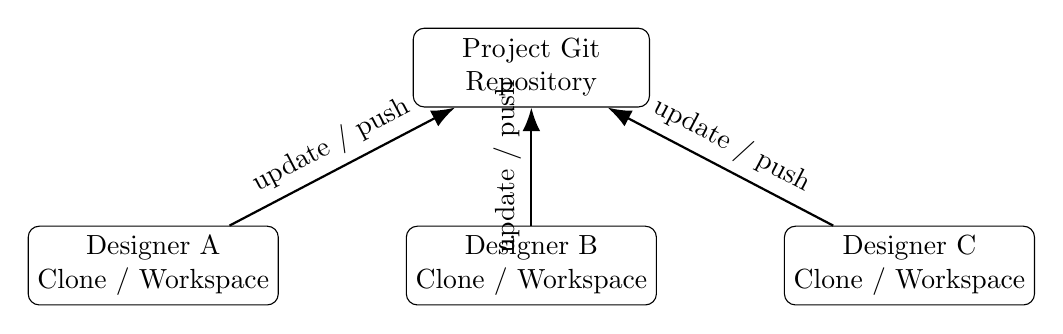
\begin{tikzpicture}[
  node distance=10mm and 15mm,
  box/.style={draw,rounded corners,align=center,minimum width=30mm,minimum height=10mm},
  arr/.style={-{Latex[length=3mm]},thick}
]
\node[box] (remote) {Project Git\\Repository};
\node[box,below left=15mm and 17mm of remote] (a) {Designer A\\Clone / Workspace};
\node[box,below=15mm of remote] (b) {Designer B\\Clone / Workspace};
\node[box,below right=15mm and 17mm of remote] (c) {Designer C\\Clone / Workspace};
\draw[arr] (a) -- node[above,sloped]{update / push} (remote);
\draw[arr] (b) -- node[above,sloped]{update / push} (remote);
\draw[arr] (c) -- node[above,sloped]{update / push} (remote);
\end{tikzpicture}
\end{center}

Private working changes remain private until committed and synchronized through the normal Git workflow. UMLCAD does not treat WebSocket broadcasting as source collaboration.

When a designer runs a Git update operation, the local source workspace changes. The local routing runtime then rebuilds or incrementally recompiles the workspace and refreshes the browser's evaluated CAD state.

\section{Concurrency and Isolation}

The system intentionally distinguishes local experimentation from source collaboration.

\begin{itemize}
    \item Uncommitted work is private to the designer's workspace.
    \item A colleague does not see another designer's trial-and-error changes merely because both are working on the same repository.
    \item Git commits are the deliberate collaboration boundary for source history.
    \item The CAD runtime evaluates the workspace actually mounted for the current designer.
    \item The same logical project may therefore have multiple private live CAD states while different designers work on different local revisions.
\end{itemize}

This design favors predictable engineering collaboration over globally broadcasting every transient experiment.

\section{Runtime and Deployment}

The initial deployment may place routing, Git, editor/LLM bridge, and CAD API infrastructure on the same physical server. They should still communicate through explicit interfaces.

For hosted execution, source code and compiler execution are isolated from the platform control plane. Docker is the first expected isolation mechanism, behind a runtime abstraction.

A typical project runtime may contain:
\begin{itemize}
    \item a designer/project workspace;
    \item a routing process or API endpoint;
    \item a Git workspace binding;
    \item source editor/LLM integration;
    \item a client to the CAD API.
\end{itemize}

The CAD implementation itself may be deployed as one or many physical service instances without changing the CAD API contract.

\section{Security and Authorization Boundary}

Authentication and authorization are external to CAD mathematics. The routing/session layer receives an authenticated authorization context and uses it to select and access the permitted project/workspace resources.

The browser is not itself a security authority. A user-interface flag such as an enabled button does not authorize an operation.

The CAD API validates engineering operations. Authorization determines who may request or modify a resource; the kernel determines whether the requested engineering state is valid. These are separate decisions.

\section{Failure and Consistency Model}

The architecture is designed so that failures do not partially corrupt accepted CAD state.

A failed process may occur because of:
\begin{itemize}
    \item source-edit failure;
    \item compilation failure;
    \item invalid geometry;
    \item unsatisfied or contradictory constraints;
    \item numerical singularity;
    \item stale semantic reference;
    \item invalid topology;
    \item engineering-rule violation.
\end{itemize}

In all such cases the accepted previous workspace/CAD state remains intact. Caches may be discarded and reconstructed without changing the semantic result.

\section{Observability and Reproducibility}

Every successful CAD result should be traceable to an immutable identity set consisting of:
\begin{itemize}
    \item project identifier;
    \item source revision;
    \item framework/kernel version;
    \item build identity;
    \item artifact hashes;
    \item semantic-manifest version;
    \item diagnostics summary.
\end{itemize}

A CAD result must therefore be reproducible from declared inputs. Server-local caches are optimization data and do not replace those inputs.

\section{Non-Goals}

The following are explicitly outside the core UMLCAD framework/kernel:
\begin{itemize}
    \item browser UI implementation;
    \item WebSocket transport;
    \item Git implementation;
    \item GitHub or another Git host's authentication UI;
    \item LLM provider implementation;
    \item Docker APIs;
    \item a mandatory desktop client;
    \item dependence on a particular commercial CAD application's object model.
\end{itemize}

In particular, the framework must not become an OCCT-style application framework merely to obtain visualization or interaction. Established external formats and mathematical libraries may be used as implementation tools where appropriate, but they must not force their complete object model into UMLCAD's public architecture.

\section{Design Principles to Preserve During Implementation}

\begin{enumerate}
    \item One engineering geometry authority.
    \item Source code is the design language; generated artifacts are derived outputs.
    \item Kernel validity is independent of UI and LLM behavior.
    \item Stable semantic identity never depends on array position, screen position, or export handles.
    \item REST CAD API requests are reproducible from explicit immutable inputs.
    \item Internal caches are optimizations, never hidden authorities.
    \item Incremental compilation and evaluation are first-class performance requirements.
    \item A small change should normally cause a small affected computation, but global changes may fall back to a broader rebuild.
    \item Git is durable collaboration/history; it is not the CAD interaction protocol.
    \item The browser is an application client, not the engineering authority.
    \item Human editing and LLM editing enter the same transactional source-edit pipeline.
    \item Undo/redo is process-level and independent of the text editor's local history.
    \item Physical deployment may change without changing logical contracts.
\end{enumerate}

\section{Reference Request Flow}

A representative property edit is:

\begin{enumerate}
    \item The user selects an object in the browser.
    \item The semantic manifest supplies the object's stable identity and editable property schema.
    \item The browser sends a semantic intent over WebSocket to the routing layer.
    \item The routing layer authenticates/authorizes the request according to the surrounding application security model.
    \item The routing layer asks the CAD API to validate the candidate operation against the declared base revision.
    \item If the operation is acceptable, the routing layer asks the human editor or LLM to create the corresponding source change.
    \item The changed source is compiled incrementally where possible.
    \item The CAD kernel incrementally evaluates the affected dependency graph and solves affected constraints.
    \item The final candidate passes the full required validation pipeline.
    \item The process becomes an accepted workspace revision and produces updated semantic/artifact outputs.
    \item The routing layer sends the result to the browser.
    \item The designer may continue experimenting privately or create a Git commit when the change is ready for collaboration.
\end{enumerate}

\section{Conclusion}

UMLCAD V5 is intentionally structured as a CAD computation platform rather than as a GUI-centered CAD application. The browser provides interaction; the routing layer orchestrates; Git provides durable source collaboration; the editor and LLM modify source; and the UMLCAD framework and kernel provide the engineering computation authority.

The central interface is the CAD API. Its RESTful/stateless contract allows multiple deployments, caching, horizontal scaling, and future process isolation while keeping the CAD semantics independent of the transport. Incremental compilation and incremental CAD evaluation provide the performance needed for interactive changes without coupling the kernel to Git or requiring a full-project rebuild for every operation.

\end{document}
